\documentclass[twocolumn]{article}
\usepackage{tikz}
\usepackage{graphicx}
\usepackage[utf8]{inputenc}
\usepackage{hyperref}
\usepackage{natbib}
\usepackage{amsmath}
\usepackage{amsfonts}
\usepackage{titlesec}
\usepackage{subcaption}
\usepackage{graphicx}
\usepackage{float}
\usepackage{enumerate}
\usepackage{algorithm}
\usepackage{algpseudocode}


\usetikzlibrary{matrix}

\newcommand{\aetitle}{Minimum Vertex-Coloring Algorithms} % Title of the report
\newcommand{\studentOne}{Mathew Smith} % Name 1

\titleformat*{\section}{\large\bfseries}
\titleformat*{\subsection}{\normalsize\bfseries}
\titleformat*{\subsubsection}{\small\bfseries}

\newtheorem{experiment}{Experiment}


\begin{document}

\input{ae_title}

\begin{abstract}
	Exact, heuristic and approximate methods of solving the minimum vertex cover problem are explored and evaluated. In particular, the quality of the approximations of the DSatur and SplitColoring algorithms are compared against the exact results of an ILP formulation. The impacts of additional algorithm engineering techniques such as pre-processing and parallelisation on the runtimes of these algorithms is also evaluated. It is found that on average DSatur provides very close to optimal colorings with very fast runtimes. The optimality and runtime of SplitColor are less favourable, but it has the advantage of providing a constant-factor approximation.
\end{abstract}


\section{Introduction}
Vertex coloring is an important problem in graph theory and computer science. On the one hand, it is a quintessential NP-complete problem; among Karp's 21 problems. On the other hand, it has wide reaching applications; many real world problems involving scheduling or avoiding conflicts can be modelled as graph coloring problems. In this report, algorithm engineering techniques for effectively computing minimum vertx colorings will be explored. There are special cases where exact polynomial algorithms exists, for example by the four-color-theorem, all planar graphs can be 4-colored, and triangle-free planar graphs can be 3-colored by Grötsch's theorem. In general however, the problem remains hard and it is this general case that will be the focus.

In section 2 the minimum vertex colorig problem will be defined, and the basic methods that will be evaluated introduced; Integer-Linear-Programming, Greedy-Coloring, and Split-Coloring. Section 3 will go into greater detail on specific implementation details of the algorithms to be evaluated, as well as introduce pre-processing techniques which will be tested. Section 4 describes the experimental setup and presents the results. Setion 5 concludes the report with discussion of the results.

\section{Preliminaries}
\subsection{Vertex-Coloring}
In the  vertex-coloring problem, the goal is to find an assignment of colours to vertices such that no adjacent vertices are assigned the same colour. In the minimum vertex-coloring problem, the goal is to find such an assignment using the minimum number of unique colors. Formally, for an undirected graph $G = (V, E)$, a coloring is a function
\begin{align}
	&c : V \rightarrow \{1, \dots, k\} \\
	\intertext{for some integer $k$ such that}
	&\forall (u, v) \in E : c(u) \neq c(v)
\end{align}
A minimum vertex-coloring then is such a function $c$ having the minimum value of $k$ for which (2) holds. 

The smallest number of colours needed to color a graph is called its \emph{chromatic number}, denoted $\chi(G)$. When certain properties of a graph are known, some upper bounds on $\chi(G)$ can be derived. The highest possible value of $\chi(G)$ is $|V|$ and is the case for all complete graphs. $\chi(G) = 1$ is only possible for edgeless graphs. A graph can always be colored with one more color than the degree of its highest degree vertex: $\chi(G) \leq \Delta(G) + 1$.
\begin{figure}[H]
\centering
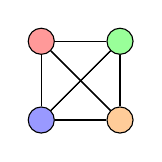
\begin{tikzpicture}[align=center, node distance=10mm, main/.style = {draw, circle, scale = 1}]
	\node[main, fill = red!40] (1) [] {};
	\node[main, fill = blue!40] (2) [below of = 1] {};
	\node[main, fill = green!40] (3) [right of = 1] {};
	\node[main, fill = orange!40] (4) [below of = 3] {};
	\draw[] (1) -- (2);
	\draw[] (1) -- (3);
	\draw[] (1) -- (4);
	\draw[] (2) -- (3);
	\draw[] (2) -- (3);
	\draw[] (2) -- (4);
	\draw[] (3) -- (1);
	\draw[] (3) -- (2);
	\draw[] (3) -- (4);
	\draw[] (4) -- (1);
	\draw[] (4) -- (2);
	\draw[] (4) -- (3);
\end{tikzpicture} \hspace{1cm}
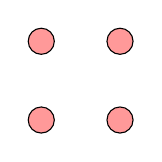
\begin{tikzpicture}[align=center, node distance=10mm, main/.style = {draw, circle, scale = 1}]
	\node[main, fill = red!40] (1) [] {};
	\node[main, fill = red!40] (2) [below of = 1] {};
	\node[main, fill = red!40] (3) [right of = 1] {};
	\node[main, fill = red!40] (4) [below of = 3] {};
\end{tikzpicture} \hspace{1cm}
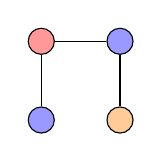
\begin{tikzpicture}[align=center, node distance=10mm, main/.style = {draw, circle, scale = 1}]
	\node[main, fill = red!40] (1) [] {};
	\node[main, fill = blue!40] (2) [below of = 1] {};
	\node[main, fill = blue!40] (3) [right of = 1] {};
	\node[main, fill = orange!40] (4) [below of = 3] {};
	\draw[] (1) -- (2);
	\draw[] (1) -- (3);
	\draw[] (3) -- (4);
\end{tikzpicture}
\caption{From left to right, complete graph: $\chi(G) = |V|$, edgeless graph: $\chi(G) = 1$, and a (non-optimal) coloring of size $\Delta(G) + 1$.}
\label{fig:chromaticnumbers}
\end{figure}

The minimum vertex-coloring problem is NP-hard. The best known exact algorithm is due to Byskov and has a runtime of $O(2.4023^n)$. The best known polynomial-time approximation algorithm is due to Halldórsson, with an approximation factor within $O(n(\log \log n)^2 (\log n)^{-3})$ of $\chi(G)$. While theoretically the best available, the two mentioned algorithms are not straightforward to implement. In both cases a number of algorithms for additional esoteric problems are called upon as subroutines. In this paper, exact, approximate, and heuristic approaches will be considered which are simple and practical while delivering promising results in terms of efficiency and optimality.

\subsubsection{Integer Linear Programming}
\label{sec:ilp2}
Integer Linear Programming (ILP) is an attractive method for finding exact solutions for minimum graph-coloring. The problem can be straightforwardly modelled with a polynomial number of constraints by appealling directly to the definition of the problem. The objective function is:
\begin{align}
	&\text{min} \sum_{1 \leq i \leq H} c_i \\
	\intertext{such that all vertices are assigned exactly one color;}
	&\forall v \in V : \sum_{i = 1}^{H} x_{v, i} = 1 \\
	\intertext{adjacent vertices are not assigned the same color;}
	&\forall (u, v) \in E, i = 1, \dots, H : x_{u, i} + x_{v, i} \leq c_i \\
	\intertext{and if a vertex is assigned a color, the variable for that color is assigned.}
	&\forall v \in V, i = 1, \dots, H : x_{v, i}, w_i \in \{ 0, 1 \}
\end{align}
$H$ is an upper bound on the number of colours. Using a heuristic to provide a smaller upper bound than $|V|$ can siginficantly reduce the runtime of the solver.


\subsubsection{Split-Coloring}
\label{sec:splitcolor2}
A $q$-approximate coloring can be achieved by arbitrarilly dividing the input graph into $q$ subgraphs of roughly equal size, running an exact algorithm on each subgraph, then merging the resulting color assignments. The runtime is $O(q\alpha^{\beta n / q} + n)$ where $O(\alpha^{\beta n})$ is the runtime of the exact algorithm used, and the additional linear component corresponds to the partitioning and merge steps. While the runtime is still exponential, the reduction in runtime may be significant enough to be of value in practice. Additionally, the approximation factor is constant with respect to $n$, unlike the best known polynomial-time approximation algorithm. Pseudocode for SplitColor is provided in algorithm \ref{alg:splitcolor}.

\begin{algorithm}
	\caption{Split-Color Approximation Algorithm}
	\begin{algorithmic}
		\Function{SplitColor}{$G = (V, E), q$}
			\State \texttt{\# partition $V$ into $q$ subsets}
			\State parts $\gets$ \textsf{partition}($V, q$)
			\For{$i$ in 1 to $q$}
				\State subgraph $\gets$ \textsf{inducedSubgraph}(part)
				\State solutions[$i$] $\gets$ \textsf{ILP}(subgraph)
			\EndFor
			\State \texttt{\# merge solutions by incrementing} 
			\State \texttt{\# the color id's by the number of} 
			\State \texttt{\# colors encountered in previous}
			\State \texttt{\# solutions.}
			\State solution $\gets$ \textsf{merge}(solutions)
			\State \Return solution 
		\EndFunction
	\end{algorithmic}
	\label{alg:splitcolor}
\end{algorithm}

\subsubsection{Greedy-Coloring}
Greedy-coloring is a popular heuristic approach for graph coloring. Vertices are considered in some order, each being assigned the color with the lowest index that has not been assigned to any of its neighbours. This approach is very fast, running in $O(|E|)$ time in its most simple form, and often yields colorings close to $\chi(G)$. The quality of the coloring however is heavily dependent on the ordering. For example, figure \ref{fig:greedybipart} shows how ordering the nodes in a bipartite graph such that nodes in the same partition are sequential yields a minimal coloring, while another ordering yields a significantly worse coloring. As such, variants of greedy-coloring exist which attempt to order the vertices in a way that increases the likelihood of a quality coloring.

\begin{figure}[H]
\centering
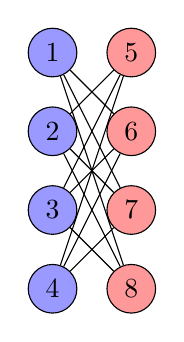
\begin{tikzpicture}[align=center, row sep = 10mm, column sep = 40mm, main/.style = {draw, circle}]
	\node[main, fill = blue!40] (1) {1};
	\node[main, fill = blue!40] (2) [below of = 1] {2};
	\node[main, fill = blue!40] (3) [below of = 2] {3};
	\node[main, fill = blue!40] (4) [below of = 3] {4};
	\node[main, fill = red!40] (5) [right of = 1] {5};
	\node[main, fill = red!40] (6) [right of = 2] {6};
	\node[main, fill = red!40] (7) [right of = 3] {7};
	\node[main, fill = red!40] (8) [right of = 4] {8};
	\draw[] (1) -- (6);
	\draw[] (1) -- (7);
	\draw[] (1) -- (8);
	\draw[] (2) -- (5);
	\draw[] (2) -- (7);
	\draw[] (2) -- (8);
	\draw[] (3) -- (5);
	\draw[] (3) -- (6);
	\draw[] (3) -- (8);
	\draw[] (4) -- (5);
	\draw[] (4) -- (6);
	\draw[] (4) -- (7);
\end{tikzpicture} \hspace{1cm}
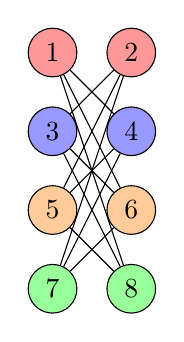
\begin{tikzpicture}[align=center, row sep = 10mm, column sep = 40mm, main/.style = {draw, circle}]
	\node[main, fill = red!40] (1) {1};
	\node[main, fill = blue!40] (2) [below of = 1] {3};
	\node[main, fill = orange!40] (3) [below of = 2] {5};
	\node[main, fill = green!40] (4) [below of = 3] {7};
	\node[main, fill = red!40] (5) [right of = 1] {2};
	\node[main, fill = blue!40] (6) [right of = 2] {4};
	\node[main, fill = orange!40] (7) [right of = 3] {6};
	\node[main, fill = green!40] (8) [right of = 4] {8};
	\draw[] (1) -- (6);
	\draw[] (1) -- (7);
	\draw[] (1) -- (8);
	\draw[] (2) -- (5);
	\draw[] (2) -- (7);
	\draw[] (2) -- (8);
	\draw[] (3) -- (5);
	\draw[] (3) -- (6);
	\draw[] (3) -- (8);
	\draw[] (4) -- (5);
	\draw[] (4) -- (6);
	\draw[] (4) -- (7);
\end{tikzpicture}
\caption{Two different colorings of a bipartite graph resulting from greedy-coloring with two different orderings.}
\label{fig:greedybipart}
\end{figure}


\section{Algorithms \& Implementations}
In this section, specifics of the algorithms to be evaluated will be presented along with relevant details on their implementations. The algorithms have been implemented in Julia v1.5\footnote{https://julialang.org/}. The \textsf{LightGraphs.jl}\footnote{https://github.com/JuliaGraphs/LightGraphs.jl} library, based on adjacency matrices, was used for graph representations.

\subsection{ILP}
The ILP formulation used exactly matches what was presented in section \ref{sec:ilp2}. To improve peformance, $\Delta(G)$ (the maximum degree of $G$) is provided as an upper bound on the number of colors ($H$). Preliminary tests revealed that not providing such an upper bound, and instead setting $H = |V|$, results in very long runtimes even on the smaller test instances. As such, the impact of this upper bound will not be a part of the experimental evaluation. Such an experiment would be very time consuming only to prove an obvious result. Given the simplicity of computing $\Delta(G)$, providing such an upper bound should be taken as a necessity for this ILP formulation. The ILP was formulated in the \textsf{JuMP.jl}\footnote{https://github.com/jump-dev/JuMP.jl} optimisation library, and the CBC\footnote{https://www.coin-or.org/Cbc/} solver was used to solve the models.

\subsection{SplitColor}
SplitColor is implemented as described in section \ref{sec:splitcolor2} and in algorithm \ref{alg:splitcolor}. The ILP implementation described above is called to compute the exact solutions to the subgraphs. 

Because the solutions to the subgraphs are computed independently, Split-Color is an ideal candidate for parallelisation. The \emph{work} $W$ is $O(q\alpha^{\beta n / q} + n)$, and the \emph{depth} $D$ is $O(\alpha^{\beta n / q} + n)$, resulting in a parallelised runtime of $T_p = O(\frac{q}{p}\alpha^{\beta n / q} + n)$: the maximal benefit is achieved when $p = q$, at which point $T_q = D$.

\subsection{DSatur}
DSatur is a variant of the greedy-coloring method. The name comes from the use of the \emph{saturation degree}: the number of neighbors of a vertex that have already been colored, to decide which vertex to color next. Pseudocode for DSatur is provided in algorithm \ref{alg:dsatur}. In the worst case there will be $O(n^2)$ key updates to the queue (e.g. in the case of a complete graph: everytime a node is colored, the saturation degree of all not-yet colored nodes will be increased). The queue used is based on a self-balancing binary search-tree. As such, initial creation of the queue takes $O(n\log n)$ time and key updates take $O(\log n)$ time resulting in an overall runtime in $O(n\log n + n^2\log n)$. While in general DSatur might produce arbitrarily bad (while still being valid colorigs) solutions, it has been shown to produce exact solutions for bipartite, cycle, and wheel graphs, and has been shown empirically to produce significantly better colorings than greedy-coloring with arbitrary orderings on average.

\begin{algorithm}
	\caption{DSatur Heuristic Algorithm}
	\begin{algorithmic}
		\Function{DSatur}{$G = (V, E)$}
			\State \texttt{\# queue implemented as a max-heap.}
			\State queue $\gets$ $\{ (v, 0) : v \in V \}$
			\While{queue is not empty}
				\State $v \gets$ \textsc{dequeue(queue)}
				\State \texttt{\# select the minimum color not}
				\State \texttt{\# assigned to $v$'s neighbors.}
				\State $v.color$ $\gets$ \textsf{firstAvailableColor(v)}
				\For{$u \in v.neighbors$}
					\State \texttt{\# increment the saturation degree} 
					\State \texttt{\# of not-yet colored neighbors.}
					\State queue[$u$] += 1
				\EndFor
			\EndWhile
		\EndFunction
	\end{algorithmic}
	\label{alg:dsatur}
\end{algorithm}

\subsection{Pre-Processing}
A vertex $v$ \emph{dominates} $u$ if the neighborhood of $v$ is a superset of $u$ (see figure \ref{fig:dominates}). If this is the case, $u$ can be removed from the graph before coloring, then assigned the same coloring as $v$. Searching for dominated nodes can be achieved in $O(n^3)$ time. Pseudocode for finding dominated vertices is provided in algorithm \ref{alg:dominated}. With the set of dominated vertices in hand, pre-processing is completed by removing those vertices from the graph, and creating a mapping from dominated to dominating vertices. The mapping can then be used to derive the coloring for the original graph from that of the reduced graph. Reducing the size of the input graph by removing dominated vertices will be evaluated as a pre-processing step to reduce the runtime of the ILP.

\begin{figure}[H]
\centering
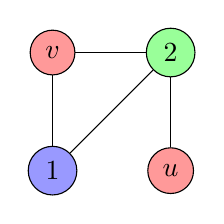
\begin{tikzpicture}[align=center, node distance=15mm, main/.style = {draw, circle, scale = 1}]
	\node[main, fill = red!40] (1) [] {$v$};
	\node[main, fill = blue!40] (2) [below of = 1] {1};
	\node[main, fill = green!40] (3) [right of = 1] {2};
	\node[main, fill = red!40] (4) [below of = 3] {$u$};
	\draw[] (1) -- (2);
	\draw[] (1) -- (3);
	\draw[] (3) -- (4);
	\draw[] (3) -- (2);
\end{tikzpicture}
\caption{$v$ dominates $u$: $v$'s neighbors are a superset of $u$'s.}	
\label{fig:dominates}
\end{figure}

\begin{algorithm}
	\caption{Algorithm to find dominated vertices for pre-processing}
	\begin{algorithmic}
		\Function{DominatedVertices}{$G = (V, E)$}
			\State dominated $\gets$ $\emptyset$
			\For{$u, v \in V \times V$}
				\If{$u.neighbors \subset v.neighbors$}
					\State dominated[u] $\gets$ $v$
					\For{$w, x \in$ dominated}
					\State \texttt{\# $v$ takes over any vertices} 
					\State \texttt{\# that $u$ dominated.}
						\If{$x = u$}
							\State dominated[$w$] $\gets$ $v$
						\EndIf
					\EndFor
				\EndIf
			\EndFor
			\State \Return dominated
		\EndFunction
	\end{algorithmic}
	\label{alg:dominated}
\end{algorithm}

\section{Experimental Evaluation}
The goal of the following experiments will be to answer the following questions:
\begin{enumerate}[(Q1)]
	\item How do the colorings yielded by the DSatur heuristic and Split-Color approximation compare to the optimal colorings provided by the ILP?
	\item What improvement in runtime is gained from pre-processing before running the ILP?
	\item What improvement in runtime is gained from parallelising Split-Color?
	\item What impact do different graph properties have on runtime and the size of the coloring? In particular it is expected that density, maximum degree, and the size and frequency of cliques are of importance to vertex coloring.
\end{enumerate}

\emph{To answers the above questions, all methods will be run on the same set of randomly generated graphs (described in the following subsection). ILP will be run with and without pre-processing to answers (Q2). The pre-processed version will be labeled ILP-P. SplitColor will be run with $q = 2, 4, 8$, and with $p = 1, 2, 4, 8$ to answers (Q3). Variants will be labelled SplitColor-q-p accordingly. Statistical analysis on the results with respect to certain graph properties will be run on the results of the ILP to answers (Q4).}

A timelimit of 10 minutes will be applied. If an algorithm fails to find a solution for an instance in under 10 minutes, that attempt will be labelled as failed.

\subsection{Data and Hardware}%
\label{sub:Data and Hardware}
The graphs used for testing were randomly generated using the \emph{expected degree model}. This model takes as input a vector $\omega$ of length $|V|$, with $\omega_v$ corresponding to the expected degree of vertex $v$. For each graph, $\omega$ was generated by sampling a normal distribution for a specific value of $\mu$, and $\sigma = \mu / 2$. This way, graphs were generated with a predictable average degree, which is an important indicator for the vertex coloring problem, while having sufficient variations between vertices and graphs to allow the algorithms to encounter a variety of structures. Graphs are grouped into sets based on the number of nodes, and subsets based on their expected degrees. For example, expdeg(36, 3) is the set of graphs with 36 nodes and expected degree of 3. Each such subset consists of 10 randomly generated graphs. Unless specified otherwise, runtimes and coloring-sizes will be averages across a subgroup.

The experiments were run on an Intel i5-8265u CPU at 1.6GHz with 4 cores, 8 threads, and 16GB of RAM.

\subsection{Results}%
\label{sub:Results}
As expected, the runtime of the approximation and heuristic algorithms were negligible compared to those of the ILP, where the runtime blew up for the larger graph sets. For 5 graphs in expdeg(72, 12), and 7 graphs in expdeg(72, 24), the ILP failed to find a solution in under 10 minutes. As such, the corresponding average runtimes in table \ref{tab:runtimes} are undervalued as they do not account for the failed attempts. The runtime of SplitColor-2 started to rise significantly on the largest graph set. The negligible runtime of SplitColor-8 on the same set demonstrates the significant reduction in runtime gained by partitioning.

\begin{table*}
	\centering
	\caption{Summary of runtimes in seconds. * indicates that some instances in the subgroup exceeded the 600 second timelimit; the average runtimes in such cases might be negatively skewed as larger runtimes were not counted.}
	\begin{tabular}[width=\textwidth]{|c||c|c|c|c|c|c|}
		\hline
		\textbf{graph set} & ILP & ILP-P & SplitColor-2 & Split-Color-4 & Split-Color-8 & DSatur \\
		\hline
		expdeg(36, 3)  & 0.08 & & 0.03 & 0.05 & 0.06 & 0.001 \\
		expdeg(36, 6)  & 1.13 & & 0.06 & 0.10 & 0.04 & 0.002 \\
		expdeg(36, 12) & 7.23 & & 0.13 & 0.10 & 0.06 & 0.002 \\
		expdeg(72, 6)  & 6.00 & & 0.10 & 0.07 & 0.07 & 0.003 \\
		expdeg(72, 12) & 202*  & & 1.50 & 0.15 & 0.17 & 0.007 \\
		expdeg(72, 24) & 155*  & & 40.0 & 0.33 & 0.26 & 0.016 \\
		\hline
	\end{tabular}
	\label{tab:runtimes}
\end{table*}

The size of the colorings produced by DSatur were \emph{very} close to the exact colorings. On average, the difference between the exact coloring and that provided by DSatur was less than 1. The SplitColor approximations were much larger, although it can be seen in figure \ref{fig:colorings} that in practice the approximation factor appears to grow sublinearly with $q$.

\begin{figure*}
	\centering
	\caption{Average number of colors per graph set for each method}
	\includegraphics[width=0.8\textwidth]{exp1_colors.pdf}
	\label{fig:colorings}
\end{figure*}

The experiments showed that the benefits of parallelising SplitColor are not emphatic. Figure \ref{fig:splitcolor}, which visualises runtimes for $q = 8$ and $p = 1, 2, 4, 8$, shows that performance is volatile across the varyious graph sets. The 8 core variant is more consistent in its runtime across graph sets, but there is no clear speed advantage. Perhaps larger test instances are necessary in order converge on a clear benefit from parallelisation.

\begin{figure*}
	\centering
	\caption{Comparison of runtimes of SplitColor-8 with different levels of parallelism. SplitColor-8-$p$ corresponds to running with $p$ cores.}
	\includegraphics[width=0.75\textwidth]{splitcolor_par.pdf}
	\label{fig:splitcolor}
\end{figure*}

The results of the preprocessing method were promising. ILP-Preprocessed was compared against ILP for graph sets expdeg(72, 6) and expdeg(72, 12). As can be seen in figure \ref{fig:preprocess}, notable decreases in runtime were achieved. On average, preprocessing was able to reduce the size of the input graph by 9 vertices.

\begin{figure*}
	\centering
	\caption{Comparison of runtimes of ILP with and without preprocessing.}
	\includegraphics[width=0.75\textwidth]{preprocessing.pdf}
	\label{fig:preprocess}
\end{figure*}

Running a linear regression model on the results with the runtimes of ILP as the independent variable and the graph properties of density, maximum degree, and maximum clique, and number of colors as dependents revealed unsurprisingly that graph density has a significant positive correlation with runtime. More interesting is that maximum degree had a slightly \emph{negative} coefficient of -5, while having an the same $r^2$ of 0.24 as density, suggesting that the impact on runtime is noteworthy. This negaive coefficient appears to be counter to intuition: a higher degree graph is likely to require a larger coloring (though not necessarily, say in the case of a bipartite graph), and it seems reasonable to expect that a larger coloring would require more time. An explanation could be that when a high degree vertex is colored, that color is ruled out for a large number of vertices, making the subsequent coloring devision for those vertices slightly easier. This is further verified by the negative coefficient for colors. Further justification for this might be that, once a large number of colors are already in play, there are more degrees of freedom for coloring new vertices without increasing the coloring size, making decisions easier. Table \ref{tab:stats} summarises these results.

\begin{table}[H]
	\centering
	\caption{Key results of a linear regression model on graph properties with runtime as the independent variable.}
	\begin{tabular}{|c|c|c|}
		\hline
		property   & coefficient & $r^2$ \\
		\hline
		density    & 2312 & 0.24  \\
		max degree & -5   & 0.24  \\
		max clique & -89  & -0.04 \\
		colors     & -37  & 0.12  \\
		\hline
	\end{tabular}
	\label{tab:stats}
\end{table}


\section{Discussion and Conclusion}
Overall, the experiments have shown that it is possible to compute both exact and approximate minimum vertex colorings using uncomplicated methods. Runtimes of the exact ILP will likely become infeasible on large graphs, but the preprocessing technique of removing dominated vertices showed promise, and surely preprocessing steps can be taken to reduce runtime. Additionally, methods of reducing the number of constraints could be explored. The performance of DSatur was extremely impressive. Runtimes are negligible while the resulting colorings were very close to optimal. Theoretically it could produce an arbitrarily bad coloring, however across the 60 graphs tested it remained very close to optimal, demonstrating that such a bad solution is unlikely. Comparitavely the performance of SplitColor was not compelling. The approximations were notably worse than DSatur. The main appeal of SplitColor will be in cases where a fixed upper bound on the quality of the solution is absolutely necessary.

\bibliographystyle{abbrvnat}

\end{document}
